\documentclass[11pt]{article}
\usepackage{amsmath, amssymb, amsthm}
\usepackage[retainorgcmds]{IEEEtrantools}

\usepackage{tikz}
\usetikzlibrary{intersections, decorations.pathreplacing}

\usepackage{fancyhdr}

%Listings stuff
\usepackage{listings}
\usepackage{lstautogobble}
\usepackage{color}

\definecolor{gray}{rgb}{0.5,0.5,0.5}
\lstset{
basicstyle={\small\ttfamily},
tabsize=3,
numbers=left,
numbersep=5pt,
numberstyle=\tiny\color{gray},
stepnumber=2,
breaklines=true,
boxpos=t
}

%Format stuff
\pagestyle{fancy}
\headheight 35pt

%Header info
\chead{\Large \textbf{Stable Matching}}
\lhead{}
\rhead{}

\begin{document}
\section{Problem}
	Given two sets $M$ of ``men'' and $W$ of ``women'', where for each $m \in M$ and $w \in W$, there exists a complete sequence of preferences of members of the other set, find a mutually agreeable perfect matching.
	
	\subparagraph{Stability} Mutually agreeable in this context is defined to be a matching with no \textbf{instability}. An unstable matching is defined as one with at least 1 pair of matches $(m, w)$ and $(m', w')$ such that $m$ prefers $w'$ to $w$ and $m'$ prefers $w$ to $w'$. In this instance, all parties involved have an incentive to work outside the system and ``elope''.
	
	Consider the following diagram:
	
	\begin{center}
	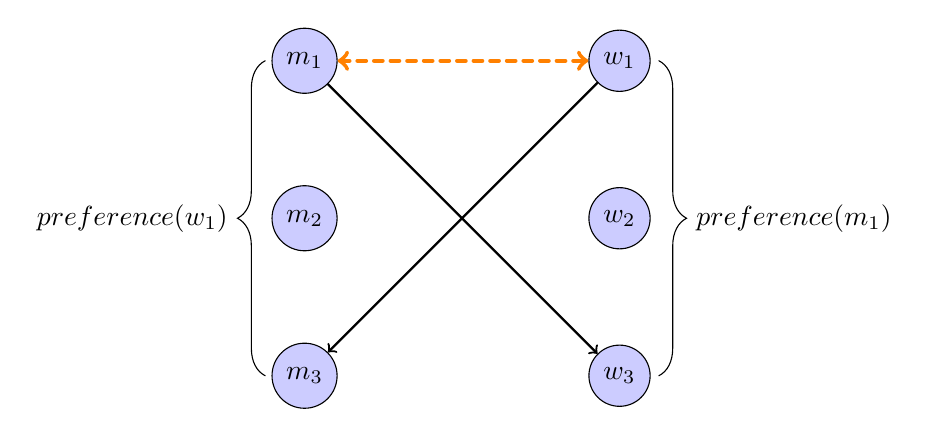
\begin{tikzpicture}
		[scale=2,line cap=round,
		%Styles
		axes/.style=,
		important line/.style={very thick},
		information text/.style={rounded corners,fill=red!10,inner sep=1ex},
		dot/.style={circle,inner sep=1pt,fill,label={#1},name=#1},
		main node/.style={circle,fill=blue!20,draw}			
		]
		
		%Colors
		\colorlet{anglecolor}{green!50!black}	%angle arcs/lines
		
		%The graphic
		
		\node[main node] (M1) at (0, 0) {$m_1$};
		\node[main node] (M2) at (0, -1) {$m_2$};
		\node[main node] (M3) at (0, -2) {$m_3$};
		
		\node[main node] (W1) at (2, 0) {$w_1$};
		\node[main node] (W2) at (2, -1) {$w_2$};
		\node[main node] (W3) at (2, -2) {$w_3$};
		
		\path[->, thick]
			(M1)	edge	(W3)
			(W1)	edge	(M3);
		
		\path[<->, dashed, ultra thick, orange]
			(M1)	edge	(W1);
			
		\draw[decorate,decoration={brace,amplitude=10pt,mirror}] (-.25, 0) -- node[left=10pt] {$preference(w_1)$} (-.25, -2);
		
		\draw[decorate, decoration={brace,amplitude=10pt}] (2.25, 0) -- node[right=10pt] {$preference(m_1)$} (2.25, -2);
	\end{tikzpicture}
	\end{center}
	In this case, because $m_1$ and $w_1$ mutually prefer each other to their currently matched partners, the matching is instable.
	
\section{Algorithm}
	The Gale-Shapley algorithm (1962) computes a perfect stable matching for the problem in polynomial (technically linear) time.
	
	\begin{lstlisting}[autogobble=true,mathescape]
		Initialize all m $\in$ M and w $\in$ W to free
		while $\exists$ free m who still has a woman w to propose to:
			if w is free:
				engage (m, w)
			else:
				let m' be current partner of w
				if w prefers m to m':
					free m'
					engage (m, w)
	\end{lstlisting}
	
	 Essentially, the men iteratively take turns proposing to women by order of preference, and the women can reject, accept, and switch partners based on their preferences. Note that while the solution is stable, it may not necessarily produce an optimal matching from the women's point of view, because while the men have the entire set of women to choose from, the women only get to choose between a limited subset of the men at any given time.

%	\begin{center}
%	\begin{tikzpicture}
%		[scale=3,line cap=round,
%		%Styles
%		axes/.style=,
%		important line/.style={very thick},
%		information text/.style={rounded corners,fill=red!10,inner sep=1ex},
%		dot/.style={circle,inner sep=1pt,fill,label={#1},name=#1}			
%		]
%		
%		%Colors
%		\colorlet{anglecolor}{green!50!black}	%angle arcs/lines
%		
%		%The graphic
%	\end{tikzpicture}
%	\end{center}

%	\begin{figure}[htb]
%		\centering
%		\includegraphics[width=0.8\textwidth]{filename.eps}
%		\caption{Caption.}
%		\label{fig:figure}
%	\end{figure}

%		\def\enotesize{\normalsize}
%		\theendnotes
\end{document}